다음 그림에서 점 $\mathrm{O}$는 둔각삼각형 $\mathrm{ABC}$의 외심이다. $\angle\mathrm{AOB} = 40^\circ$, $\angle\mathrm{BOC} = 50^\circ$ 일 때, $\angle\mathrm{ABC}$의 크기는 몇 도인지 구하여라.

\begin{figure}[h]
\centering
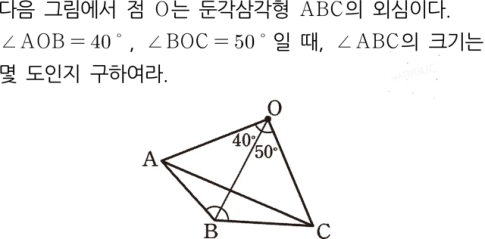
\includegraphics[width=0.3\textwidth]{plain0_problem_07_figure.png}
\end{figure}
